% !TeX spellcheck = en_US
\section{Perceived Quality of UGV}
\label{sec:210_quality_assessment}
A central aspect of content-adaptive media streaming is to gain a detailed understanding of the perceived quality for the viewer.
Quality is defined as the "[...] evaluated excellence or goodness [...]" or "[...] the degree of need fulfillment [...]"~\cite[4]{Qualinet2013}.
The focus lies on the discussion of quality as it is perceived for \ac{UGV}, as well as existing methods to determine it.
\subsection{Overview of the Video Streaming Process}
\label{sec:210_streaming_process}
The process of \ac{UGV} streaming, from the capturing of a video until the playback on a mobile device, is an extension of the recording steps proposed by Jang et al.~\cite{Jang2016}.
To determine the perceived quality, influencing factors from all process steps (see Figure~\ref{fig:210_recordingprocess}) need to be considered.
\begin{figure}[tbh]
\centering
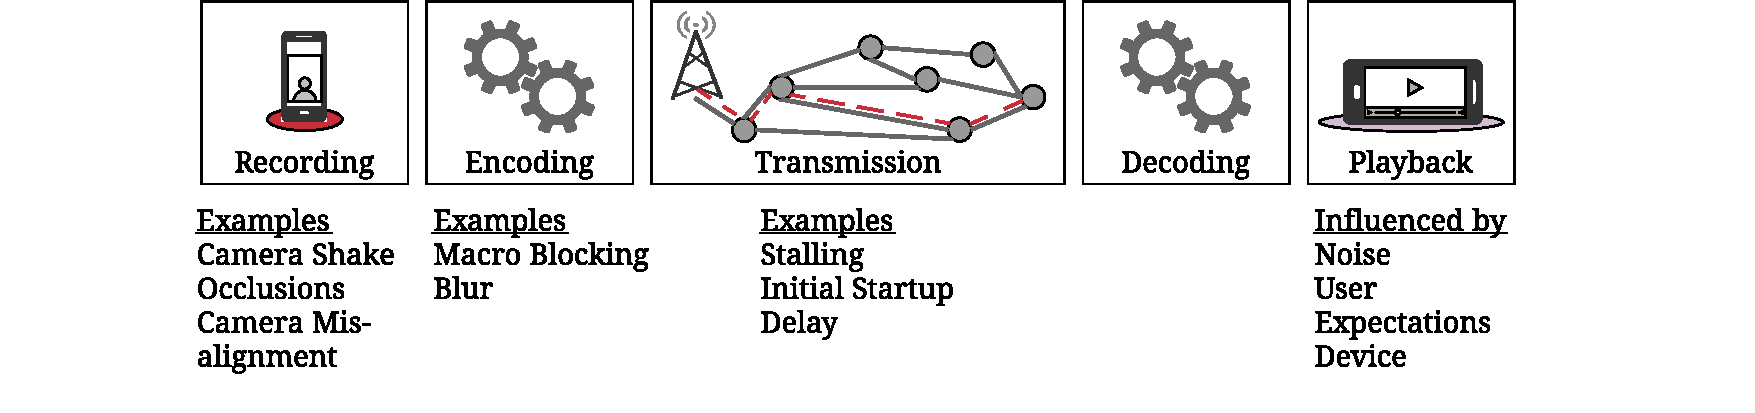
\includegraphics[width=\linewidth]{gfx/200_Background/Recording_Process}
\caption[Video streaming process]{Video streaming process and its problems as understood in this thesis.}
\label{fig:210_recordingprocess}
\end{figure}

It starts on the video recording side, where the users' actions influence the perceived quality.
The process continues over the compression of the video (encoding) and the transfer over a communication network such as the Internet.
It ends at the viewer's side with the decoding and rendering of the video on a display.
\subsubsection{Recording Step}
The first step is the recording of a real-world scene by a non-professional cameraman.
In this thesis, it is assumed that the recording device is a smart mobile device as discussed earlier. 

There are two essential differences between professional productions and \ac{UGV}: 1) the skills of recording users and 2) the equipment used for capturing a video.
Professional equipment consists of cameras, which include physical or digital stabilization mechanisms to create stable video frames.
These mechanisms allow a controlled focus, panning and tilting of the camera without any disturbing (unintended) motion to occur.
Professional cameras are mounted on tripods, dollies or cranes to support a broad range of applications.
Further optical and digital mechanisms help to capture videos, e.g., adjustable lenses to capture different distances. 

In contrast to professional cameras, today's smartphones have cheap lenses with large apertures causing degraded quality in low light settings~\cite{Dialogic2009}.
Also, sensors need to comply to low energy consumption requirements, making recorded frames less attractive.
As a result, the recorded videos are not of the same quality as if produced by professional cameras. 

Also, most degrading effects occur due to the lacking skill of users.
Especially the degradations caused by camera shakes, harmful occlusions and camera misalignments are to be mentioned.
\emph{Camera shake} is caused by uncontrolled movements of the recording user due to the lack of a stabilizing tripod.
If such movements occur continuously with varying directions, they are named camera shakes.
In contrast to camera shakes, intended motions of the camera include tilting and panning.
Tilting describes motion about the horizontal axis of the camera, whereas panning occurs about the vertical axes.
In contrast to shake, these intended forms of motion do not include repeated direction changes~\cite{Ward2003}.
Some recent high-end smartphones compensate unintended motion using optical image stabilization\footnote{http://www.cultofmac.com/390139/optical-image-stabilization-iphone/; Visited on: 09/15/2016}.
An extra gyroscope is used to control movements of an adjustable camera to compensate for unintended movements. 
It works in the range of tenths of millimeters for each exposure~\cite{Karpenko2011,Shin2011}.

\emph{Harmful occlusions}, also termed as occultations, depict that a foreground object blocks the view of a background object, which is in the \ac{RoI} of a video frame.
The \ac{RoI} illustrates that such an occlusion is perceived as distracting if the viewer is interested in watching the background object.
Other occlusions may not be perceived as distracting as they are a natural part of a scene.
A harmful occlusion often occurs in \ac{UGV} as users move while recording, and objects cross the line of sight of a recording device.

\emph{Camera misalignments} represent the case when smart mobile devices do not capture the commonly agreed \ac{AoI}, e.g., the stage during a concert.
Misalignments start from slightly drifting away from the \ac{RoI}~\cite{Bowen2013} to its worst form, where the recording does not capture the \ac{RoI} at all. 
A second type of misalignment addresses the orientation along the axis describing the device's viewing direction (z-axis). 
Users may change from a perfectly aligned orientation to slightly tilted recordings.
This tilt is measured as the difference of the recorded plane (consisting of horizontal and vertical axes) to the reference plane of a scene.  

\subsubsection{Encoding}
Typical compression algorithms lead to a lossy conversion of the input, which results in information loss that cannot be compensated on the decoding side.
As discussed earlier in this chapter, compression is achieved by leveraging the redundancy available in and between video frames.
Common encoding degradations address both spatial effects within a single frame and impairments reducing the perception of motion in the video~(see \cite{Jang2016,TaoLiu2010} for an overview on degradations). 
Encoding is a very resource-consuming process, which does not always achieve satisfying results on smart mobile devices.
If the resource demand is too high, this usually results in the skipping of captured frames before encoding - thus reducing the possible frame rate.
Stohr et al. conducted work illustrating this effect for the live streaming platform YouNow~\cite{Stohr2015}.
The authors show that the average and for most technologies, the highest frame rate observed is still lower than what the average human perceives as smooth motion~\cite{Kandel2013}. 
The resulting video streams are perceived as jerky (motion jerkiness), which degrades the perceived quality. 
\subsubsection{Transmission}
Degrading effects can also occur during the transmission of a video stream over a network.
Degradations consist of packet losses that result in a degraded video decoding, the initial startup delay, and \ac{stalling} effects.

In best effort delivery schemes, sent packets of a media stream can be lost or delayed so that the video receiving side cannot completely decode the video~\cite{Dialogic2009}.
Such a packet loss may affect an entire frame or only a part of its data~\cite{TaoLiu2010} and existing video encoding standards implement methods to compensate a small percentage of packet losses without significantly degrading the viewing experience~\cite{Sullivan2012,Wiegand2003}.

Besides that, user experience can be degraded due to the initial waiting phase for the video stream or frequent interruptions during playback, i.e., \ac{stalling}~\cite{Hossfeld2012}.
Both happen when network capacity is lower than the video bit rate, which implies that an in-time delivery of the video stream is not possible.
Simply said, the video is being consumed faster than it is delivered.
Recent studies show that \ac{stalling} significantly degrades the viewing experience~\cite{Hossfeld2012,Hossfeld2013,Hossfeld2014}.
\subsubsection{Playback Context}
User perception, device capabilities, and environmental conditions affect how a video stream is perceived at the receiver's side.

User perception is composed of characteristics which can be any (in)variant property of the person, which describes its demographic and socio-economic background, current emotions, or physical as well as mental constitution~\cite{Qualinet2013}.
Such characteristics can be user's viewing habits as well as disabilities such as color blindness.

The device can influence the perception by any of its features that determine the technically produced and measurable quality of the video stream~\cite{Qualinet2013}.
In the context of video playback, this addresses factors such as the decoding quality, display size, and brightness, as well as available decoders on the device.

Finally, the environmental conditions and the context describe any property of the physical, temporal, and social context of a video playback session~\cite{Qualinet2013}.
It contains lighting conditions, ambient noise or any other distraction, as well as the time of day and cost of a service.

The integration of the context during video playback for the perceived quality has attracted research initiatives that have not yet been widely accepted~\cite{Kroupi2014,Luo2008,Moorthy2012,Scholler2012}.
This area is not in the focus of this work, but the effects of using mobile devices with reduced display sizes for video playback are considered in Chapter~\ref{sec:700_VAS}.
% -  -  -  -  -  -  -  -  -  -  -  -  -  - 
\subsection{Subjective Quality Assessment}
\label{sec:210_subjective_quality}
The most reliable method to determine the quality of a video streaming session is to ask the viewers of the stream.
This method can be reproduced as large-scale subjective experiments, where multiple subjects assess the video stream's quality regarding standardized assessment scales~\cite{Winkler2008}.
Another advantage of subjective quality studies is that it can be applied to degradations occurring at any step of the video streaming process (see Section~\ref{sec:210_streaming_process} and Figure~\ref{fig:210_recordingprocess}). 

For performing a subjective quality study, multiple subjects are used to mitigate subjective preferences and retrieve a mean opinion on the quality.
The subjects conduct their judgments on standardized quality assessment scales.
Following the rules of the \ac{ITU}, the subjective experiments are conducted under controlled conditions~\cite{ITU-R2012,Winkler2009}.
Quality assessment scales discussed in this thesis include the \ac{ITU} recommendation \ac{SSCQS}~\cite{ITU-R2012}. % and \ac{ACR}~\cite{ITU-J2008}.

Judgments are then aggregated into subjective quality metrics.
In this thesis, the metrics \ac{MOS}~\cite{ITU-J800} and \ac{JND}~\cite{Watson2001} are used.
Conducted subjective experiments and resulting quality metrics build the benchmark for all objective quality metrics~\cite{Winkler2008}. 
For the interested reader, further subjective metrics are introduced by Hossfeld et al.~\cite{Hossfeld2016}, and quality assessment scales are discussed by the respective \ac{ITU} recommendations~\cite{ITU-R2012,ITU-J800}.
\subsubsection{Assessment Scales}
Subjective experiments conducted in the thesis ask users to rate the quality of video sequences one-by-one, or select the highest-quality sequence between a reference video and an impaired sequence.

Evaluations that assess the absolute quality of a video sequence individually leverage the \ac{SSCQS}, which ranges from one to five.
Here, one represents the worst quality imaginable (bad) and five the highest possible quality (excellent)~\cite{ITU-R2012}.
In a \ac{UI}, the scale is usually represented as a slider, where each integer values is annotated by the respective quality descriptions - 1: bad, 2: poor, 3: fair, 4: good and 5: excellent (see Figure~\ref{fig:210_qualityscales}).
\begin{figure}[th]
\centering
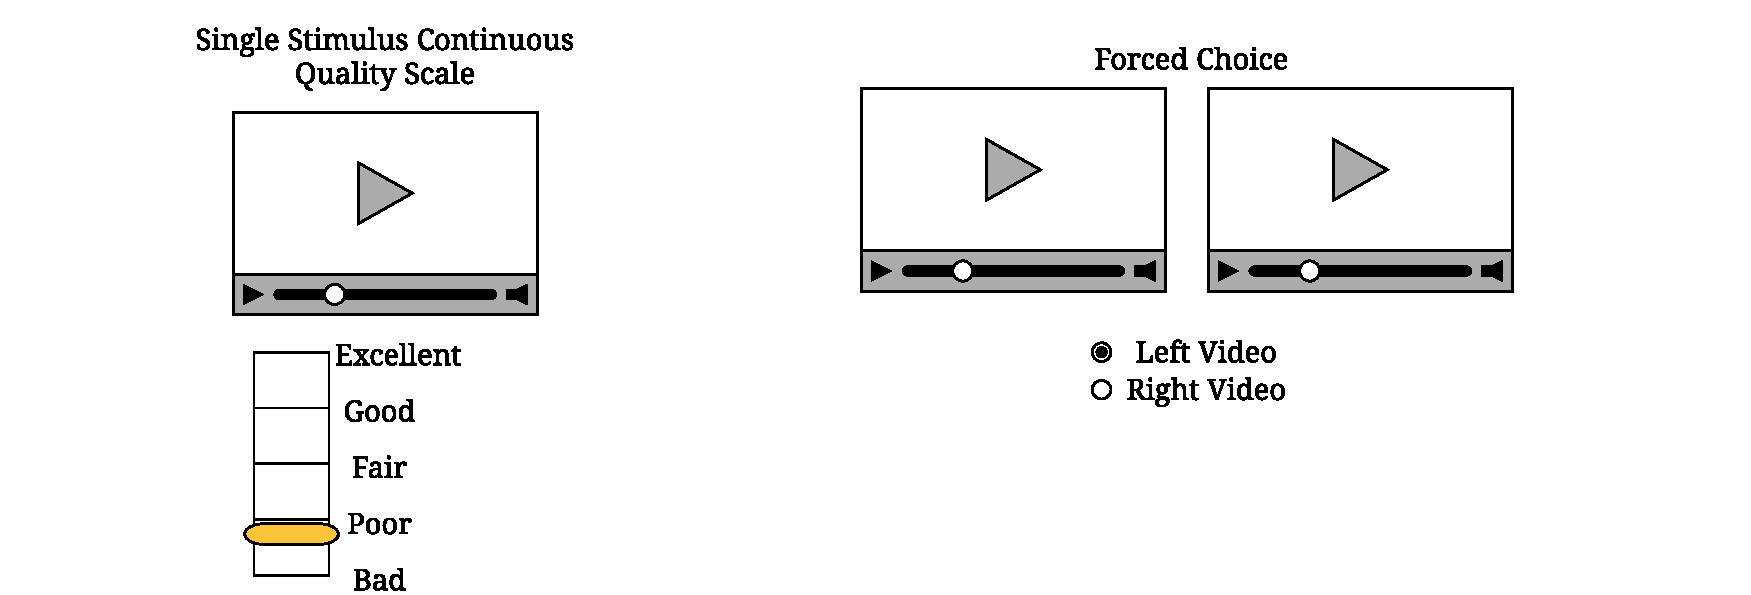
\includegraphics[width=\linewidth]{gfx/200_Background/qualityScales}
\caption[Subjective quality assessment scales]{Subjective quality assessment scales: Single Stimulus Continuous Quality Scale (SSCQS) and Forced Choice Experiment.}
\label{fig:210_qualityscales}
\end{figure}

This evaluation methodology is suitable to determine quality as perceived in real streaming sessions, as the viewer does not know in advance if a degradation is present or not.
The \ac{SSCQS} is the basis for the subjective quality metric \ac{MOS}.

A forced choice experiment (see Figure~\ref{fig:210_qualityscales}) is set up when it should be determined if a degradation can be detected in a direct comparison of two video sequences.
Instead of a continuous scale, the viewer decides which video sequence has the higher quality.
This binary decision is the basis for the \ac{JND}~\cite{Keelan2003}.
\subsubsection{Metrics}
As mentioned above, \ac{MOS} is a concept to describe the subjective perception of quality, and is calculated from the \ac{SSCQS}~\cite{Suarez2016}. 
The \ac{MOS} of a video ranges from 1 (bad) to 5 (excellent).
The \ac{MOS} is calculated as the average of the subjects ratings as
\begin{equation}
	MOS = \frac{1}{N}\sum_{i=1}^{N}r_{ij}
\end{equation}
where $N$ represents the number of assessments for a video $j$ and $i$ is the index of a subject. 
Thus, $r_{ij}$ represents a quality rating of one user for one video.

As ratings of individuals may be very diverse, a data cleaning and a rating normalization task are performed.
The data cleaning is recommended by the \ac{ITU}-R BT.500 and identifies inconsistently rating subjects. 
The procedure is discussed in the Annex B of \ac{ITU}-R BT.500 in Section 2.3.2~\cite{ITU-R2012}.

For the resulting ratings, a normalization is conducted. 
It ensures that subjective assessments are comparable and is proposed by Simone et al. and refined by Horch et al.~\cite{DeSimone2010,qualitycrowd}. 

For normalizing the ratings we calculate the value $r'_{ij}$, which is derived from the original rating $r_{ij}$ corrected by the average of ratings of the assessor $\overline{r_i}$.
Also, the mean across all assessors and video sequences $\overline{r}$ is used for normalization:
%This leads to the calculation of $r'_{ij}$  %, where each campaign represents one recorded event with several sequences.
\begin{equation}
r'_{ij} = r_{ij} - (\overline{r_i} - \overline{r}) 
\end{equation}
The \ac{MOS} aggregates all ratings by:
\begin{equation}
MOS_{j} = r_{j} =  \frac{\sum_{i=1}^{N} r'_{ij}}{N}
\end{equation}

A second quality metric is the \ac{JND}, which is determined in a forced choice experiment~\cite{Keelan2003,Watson2001}.
The \ac{JND} is an \ac{ISO} standard for the assessment of quality in images and videos.
This method tries to determine the minimum difference $\delta_{\Psi_{A,B}} = \Psi_A - \Psi_B$ between two video signals A and B, which is noticeable by a human.
$\Psi_A$ represents the perceived quality of the video $A$ and $\Psi_B$ the quality of video $B$.
The \ac{JND} can be determined using forced-choice tests in which each subject rates the same two video sequences - one being an impaired sequence and the other an unimpaired video.
The viewer does not know which of the two video sequences is unimpaired.
The order of comparisons is randomly selected and repeated several times for different subjects.
In each evaluation round, the subject has to decide which stimulus is the best. 
If a stimulus receives 75\% of the votes, it achieves a \ac{JND} of one~\cite{Thang2014}.
The generalized model is that the 
$\delta_{\Psi_{A,B}}$ is represented in \ac{JND} units as $\delta_{\Psi_{A,B}}  = \frac{12}{\pi} * arcsin(\sqrt{v})-3$, where $v$ is the fraction of votes ([0,1]) for one video~\cite{Thang2014}.
\subsection{Objective Quality Assessment}
\label{sec:210_ojective_quality}
Objective quality assessment predicts the quality an average user would perceive when watching a video sequence~\cite{Winkler2008}. 
%Metrics range from signal comparison over bit stream metrics or mapping the human perception by remodeling the \ac{HVS} into an objective metric. 
The algorithms can be divided into \ac{FR}, \ac{NR} and \ac{RR} metrics.
Video quality metrics belonging to the \ac{FR} category require a perfectly preserved reference video sequence, which is often used in conjunction with the potentially impaired test sequence~\cite{Winkler2008}.
\ac{FR} metrics detect the physical differences (pixel differences) in the two sequences easily.
The challenge is to map the detected differences to human perception to understand their impact on the perceived quality.
Since every pixel of every video frame of a sequence is compared with its reference, the processing time and required computational resources can be enormous. 
The practical usage of \ac{FR} metrics in streaming scenarios is often limited as the delivery of the unimpaired video sequence is inefficient or unrealizable.

\ac{NR} video quality assessment examines solely the test video without any need for a reference~\cite{Winkler2008}. 
The accessibility of the original video may be impractical or problematic because the output of a camera may already be compressed. 
\ac{NR} quality assessment approaches are more suitable to be used for assessing video streaming scenarios as only a single video is needed for assessment.
At the same time, these metrics achieve a significantly reduced correlation with subjective quality assessments in comparison to \ac{FR} approaches~\cite{Winkler2009}.

\ac{RR} metrics describe an intermediate approach, which does not require a reference video sequence, but solely some metric-specific features which are extracted from the reference video.
The \ac{RR} metric uses the test sequence and the extracted reference features for the quality prediction.

In the remaining section, existing objective quality metrics are described and compared.
This discussion is split into the assessment of user-generated degradations and the analysis of standardized algorithms which detect impairments induced by the compression, the transmission or the playback of the video stream.

This distinction is chosen, as the set of standardized and evaluated algorithms focuses on the effects of compression and transmission effects on the video, thus, excluding degradations occurring while recording.
\subsubsection{Recording Quality Assessment}
\label{sec:210_VideoQuality}
Degradations caused by the user's actions are termed as recording degradations.
As mentioned above in this thesis, some of the most severe degradations are discussed: camera shakes, harmful occlusions and camera misalignments.
For an extensive discussion of other degradations in \ac{UGV}, please refer to the work of Jang et al.~\cite{Jang2016}.

It is important to know that only \ac{NR} metrics can be leveraged, as no reference video is available.
The algorithms discussed for camera shake, harmful occlusion and camera misalignment assessment are thus \ac{NR} metrics.
\paragraph{Camera Shake Assessment}
Camera shake assessment on mobile recording devices is achieved by either analyzing the video or auxiliary sensor samples gathered during a recording session.
Video-based algorithms are the most prominent ones; they achieve a high reliability at the costs of a high runtime.
An early approach towards the detection of camera shakes is proposed by Campanella et al. in their work targeting at summarizing home videos automatically~\cite{Campanella2007}. 
The approach leverages the  \ac{LPC} algorithm on each video frame and compares consecutive video frames to detect occurring panning and tilting, so the horizontal and vertical movements of a camera~\cite{Nagasaka1999,Uehara2004}.
The consecutive frames are put into fixed size segments to be analyzed.
A threshold is used to filter only significant motion that is then classified as a shake using the following equation: 
\begin{equation} \label{eq:210_shakinessCampanella}
  \textit{S} = \frac{1}{N} \displaystyle\sum_{i=1}^{N} \sqrt{(pan_i - fpan_i)^2 + (tilt_i - ftilt_i)^2}
\end{equation}
Here, $N$ represents the number of frames in a video segment, $pan_i$ and $tilt_i$ are original pan and tilt values, $fpan_i$ and $ftilt_i$ are low-pass-filtered pan and tilt values. Here, $i$ represents the current frame index.
The quality impact of the detected shakes in a video segment is then determined as $Q_{CM} = \frac{S_{max}-S}{S_{max}}$.
Values for $S_{max}$ are not given by Campanella et al. - limiting the reproducibility of results~\cite{Campanella2007}.

The approach of Campanella et al. has attracted interest in the research community~\cite{Campanella2007}. 
Many of the video composition applications leverage (and slightly extend) the approach~\cite{Bano2015b,Saini2012,Shrestha2010}.
Saini et al. replace the low-pass filter preprocessing step by a median filter to better distinguish intended camera motion, i.e., pan and tilt, from camera shakes~\cite{Saini2012}.
Also, the final shake score is the sum of absolute differences of the original motion vectors and median filtered motion vectors, and follows Equation~\ref{eq:210_shakinessCampanella}. 
The score calculation is applied to a window of 100 frames and post-processed in order to normalize the values to the range of [0,1].

Abdollahian et al. introduce a  machine learning approach for the classification of camera motion~\cite{Abdollahian2010}.
On the basis of detected panning and tilting using a pixel matching approach called the Integral Template Matching, a \ac{SVM} is trained to classify shakes, blur, stability, and zooms~\cite{Dong-JunLan2003}.
On the given dataset, a classification rate of around 87.32\% is reported - but no relation to the perceived quality is given.

On the other side, auxiliary sensor-based algorithms are proposed for camera shake detection.
Cricri et al. propose to leverage the compass on smartphones and applying a low-pass filter to identify camera pan, tilt and shakes~\cite{Cricri2012}. 
The algorithm maps the real-time gathered compass sensor readings to the video. 
Next, motion detected by the compass is classified in three steps: 1) low-pass filtering of raw compass data, 2) computation of the first discrete derivative on the compass readings, and 3) a peak detection based on a predefined threshold.
Camera shake can be detected and removed in the first step by applying the low-pass filtering.
This approach only works for very short shaky segments of a video.

This work was extended by investigating the accelerometer as a source for reliably detecting camera shakes~\cite{Cricri2012}.
The underlying assumption is that frequency contributions between 10 to 20 \unit{Hz} are caused by camera shakes~\cite{Yu2007}.
The resulting algorithm leverages a high-pass filter at a frequency of 10 \unit{Hz} in all three axes of the sensor (y,y,z).
On the basis of the filtered values for each axis, the variance is calculated as $\sigma^2 x$, $\sigma^2 y$ and $\sigma^2  z$.
The median of the three values is chosen in order to avoid outliers on a single axis to impact the shake intensity measurement.

Bano et al. propose another auxiliary sensor approach, leveraging the gyroscope of smartphones~\cite{Bano2015}.
They aim at dissecting pan and tilt from the camera shakes.
In a first step, the radial component of a gyroscope sensing is computed as $G_r(t) = \sqrt{G_x(t)^2 + G_y(t)^2}$, where $G_x(t)$ represents the degree of motion sensed on the x-axis, and $G_y(t)$ the proportion on the y-axis.
A shake is then detected and stored as a binary variable $S(t)$ as
\begin{equation}
S(t) =
 \begin{cases}
 1       & \quad \text{if } G_r(t) > \beta,\\
 0       & \quad \text{otherwise}
  \end{cases}
\end{equation}
$\beta = 0.06$ is an empirically determined shake threshold. 

Liu et al.~\cite{Liu2014} propose an algorithm to classify camera motion into intended motion or unwanted motion.
They leverage similar, previously mentioned models by using the accelerometer as a source.
Similar to other approaches, these are either video- or auxiliary sensor-based, and no mapping to the perceived quality is given.
\paragraph{Harmful Occlusion Detection}
Occlusion detection is a required step in object or template tracking~\cite{Koller1994,Nguyen2001,Saravanakumar2012,Weng2006}.
Weng et al. present one example of this category~\cite{Weng2006}.
The proposed algorithm can track moving objects even in the presence of occlusions.
An object is tracked after it is annotated manually.
To track the object, a region growing segmentation approach is applied in the frames $t$, $t-1$, $t + 1$.
Similarly, a segmentation is performed on the dominant colors of the respective video frames.
An occlusion of an object is detected when the ratio of the object's area in the frame $t$ compared to $t-1$ shrinks, and similarly, its size decreases from frame $t$ to $t+1$.
Those models try to detect occlusions but give no reasoning on the impact of the occlusion on the quality.

Saini et al. propose the most promising approach when it comes to a low computational complexity and an application to \ac{UGV}~\cite{Saini2012}.
The underlying assumption is that occluding objects must be closer to the camera and thus show a lower edge density than the occluded objects, which exhibit a higher distance to the recording camera.
By continuously checking for significant differences in the edge densities in a scene, candidates for occlusions can be detected.
%Therefore, 
Each video frame is first represented in an edge representation using the Canny Edge Detector~\cite{Canny1986}.
A binary representation of a video frame is derived, which depicts an edge pixel as 1 and a non-edge pixel as 0.
A convolution matrix is applied to the binary edge representation using a unity kernel matrix $W$  (usually a matrix of ones): $I^d = I^e \odot W$ where $\odot$ represents the convolution operation.
As harmful occlusions occur at specific regions and seldom occlude the whole video frame, subblocks of the frame are constructed, where each block has a size  of $b \times c$. 
For each block, it is determined if it is occluded by calculating the sum of the edge densities and determining if it is less than the threshold $T^e$.
The authors state that $T^e$ should represent a meaningful, empirically determined value for separating foreground from background objects.
As neighboring blocks could indicate diverging statements on whether the whole frame region is occluded or not.
Then a connected component analysis is conducted, which tries to find the largest group of connected (occluded or non-occluded) blocks in a frame. 
Gaps are labeled as occluded if the majority of their neighboring blocks are occluded.
An occlusion score $S^O$ is computed by the fractional occluded region $f$ as
\begin{equation} 
f = \frac{N_{O}}{N_{Total}}
\end{equation}
where the resulting occlusion score is represented as $S^O = 1 - e^{-f}$. 
$N_{O}$ represents the blocks labeled as occluded and $N_{Total}$ the total number of blocks. 
The authors state, that for a block size of $20 * 15$ pixels an occlusion score of  more than $0.2$ can be classified as disturbing. Further information on the relation of the algorithm to the perceived quality is not given.
\paragraph{Camera Misalignment and Orientation}
Similar to the camera shake assessment, the misalignment detection can be classified into algorithms either inspecting the video or leveraging auxiliary sensor data.
An additional criterion is the detection of either misaligned recordings for a given \ac{RoI} or the issue of tilting the camera during the recording.
Most of the existing algorithms focus on camera orientation, 
but none quantifies the impact of a view not being perfectly aligned with the \ac{RoI}~\cite{Cricri2014,Saini2012}. 

Saini et al. propose a video-based algorithm for camera orientation detection relying on the distinction of horizontal to non-horizontal edges~\cite{Saini2012}.
It is assumed that the majority of edges are horizontally aligned, when a smart mobile device records in landscape mode.
Camera orientation is thus defined as a rotation of the camera around the horizontal axis of the recording device.
From an edge representation of the video frames, a \textit{Hough transform} is performed in order to detect straight lines, where $l_i$ represents the length of the $i^{th}$ line and $o_i$ is the angle in relation to the horizontal plane. 
It is assumed that a camera is tilted by less than $\pm\frac{\pi}{4}$, corresponding to $\pm45\degree$.
Thus, any higher angle describes that the respective line is noise.
The resulting orientation is $o_i$ for a line $i$, which is used for determining the camera orientation as:
\begin{equation} \label{eq:210_SainiTiltScore}
CO =  \frac{\abs*{\frac{1}{N^l} \displaystyle\sum_{i=1}^{N^l} o_i * l_i} }{\pi/4} 
\end{equation}
Here, the score is obtained on the basis of the absolute mean orientation being weighted and normalized by $\frac{\pi}{4}$ ($45\degree$). 

Cricri et al. propose a method for orientation detection by making use of auxiliary sensors (accelerometer or compass) of smartphones~\cite{Cricri2011}.
The wrong orientation is determined by analyzing the static component of accelerometer readings without any motion of the device itself.
For each intended display orientation, either landscape or portrait, a contribution to the accelerometer axis can be determined.
In a properly oriented camera, one axis should not sense any contribution to another axis, e.g., on the y-axis in the landscape orientation.
The approach of Cricri et al. leverages the low frequency accelerometer proportions by preprocessing the data using a low-pass filter at 10 \unit{Hz}.
The resulting filtered readings are used to combine the instantaneous orientations $O_I$ as 
\begin{equation}
O_I = arctan \frac{A_y}{\sqrt{(A_x)^2 + (A_z)^2}}
\end{equation}
If $O_I$ is larger than a predefined threshold $T_{O_I}$ - which represents the acceptable deviation angle - the recording is classified as the wrong camera orientation.
\paragraph{Discussion}
Except for the camera shake assessment, only a limited set of algorithms exist for detecting severe recording degradations.
All algorithms suffer from a lack of validated quality models.
Existing work does not quantify the perceived quality but solely detects a degradation. 
Thus, quality is mapped to a binary value, i.e., a low quality when a degradation is detected, and a high quality if no degradation is found.

Camera shake assessment and camera misalignment algorithms use visual and auxiliary sensor features.
These algorithms show the trade-offs between accuracy in detecting degradations and runtime.
Whereas auxiliary sensor-based algorithms are quick to process, but usually suffer from imprecise sensors.
These existing approaches neither compensate for the imprecision nor leverage visual features to support auxiliary sensor-based algorithms.

In general, it can be concluded that despite the overwhelming success of \ac{UGV}, a limited set of algorithms exist to detect degradations common in \ac{UGV}. 
%===================================================================================================================================================================
%===================================================================================================================================================================
\subsubsection{Compression and Transmission Effects}
\label{sec:210_qualitymetrics}
Instead of discussing assessment methods for single impairments such as macro blocking, comprehensive objective quality metrics are discussed~\cite{Wang2002}.
These algorithms analyze the most common and most deteriorating degradations occurring while encoding and transmitting a stream.
The section describes the objective quality assessment method \ac{PSNR}, \ac{SSIM}, \ac{VQM}, \ac{VMAF}, and \ac{V-BLIINDS}. 
\paragraph{PSNR}
To calculate the \ac{PSNR}, a pixel-by-pixel comparison of two video frames is performed that investigates the impaired frame on noise in relation to the reference frame.
Even though \ac{PSNR} can be quickly calculated, it neglects features such as the "[...] content,~[...]"~\cite[2]{Winkler2005} and "[...] viewing conditions on the actual visibility of artifacts [...]"~\cite[202]{Winkler2001}.
Thus, it shows a weak correlation with perceived quality, but the \ac{PSNR} is often used to assess the performance of video codecs and streaming applications~\cite{Suarez2016,Winkler2008}. 

The \ac{PSNR}~\cite[472]{Stathaki2011} is expressed as
\begin{equation}
PSNR = 10 \times log_{10}(\frac{L^2 \times r \times c}{\sum_{i=0}^{r-1}\sum_{j=0}^{c-1}[R(i,j)-I(i,j)]^2})	\qquad[\unit{dB}]
\end{equation}
$L$ determines the maximum pixel values, which is usually $255$ in a $8$ bit, monochrome representation of a video frame.
$i$ and $j$ represent pixel indices, $r$ represents the number of rows and $c$ the number of columns in a frame.
$R$ is the reference frame whereas $I$ represents the impaired video frame.
\paragraph{SSIM}
The \acf{SSIM} is an objective quality assessment metric that has been designed to determine the closeness of two still images~\cite{Wang2004}.
It relies on the investigation of the luminance, the contrast and the structure in the images and achieves a good correlation with subjective study experiments.
For analyzing video sequences, it neglects the impact of motion.

The \ac{SSIM} is calculated as
\begin{equation}
SSIM(R,I) = \left[l(R,I)^\alpha \times c(R,I)^\beta \times s(R,I)^\gamma \right]
\end{equation} 
where $\alpha + \beta + \gamma = 1$. 
$\alpha$, $\beta$, and $\gamma$ build weights for the individual components of the \ac{SSIM}.

The three components analyze the luminance ($l(R,I)$), the contrast ($c(R,I)$) and the structures ($s(R,I)$) of two video frames $R$ and $I$.
$R$ and $I$ are represented as array of pixel values of a gray image, where each pixel has a bit depth of 8 bit and a single channel.

The luminance component of the formula is calculated as
\begin{equation}
l(R,I)=\frac{2 \times \overline{R}  \times \overline{I} + c_1}{\overline{R}^2 + \overline{I}^2 + c_1}
\end{equation}
$\overline{R}$ is the average of frame $R$ and $\overline{I}$ is the average of frame $I$.
$c_1 = (k_1 \times L)^2$ is a stabilizing factor in cases when the averages of $R$ and $I$ are close to zero.
The authors state that $k_1$ should be a small constant $<<1$ and $L=255$ for 8 bit gray images. 

The contrast component is calculated as
\begin{equation}
c(R,I)=\frac{2 \times \sigma_R  \times \sigma_{I} + c_2}{\sigma^2_{R} + \sigma^2_{I} + c_2}
\end{equation}
Here, $\sigma_R^2$ and  $\sigma_I^2$ are the variances of $R$ and $I$.
Again, a stabilizing factor is used and calculated as $c_2 = (k_2 \times L)^2$, where $k_2 << 1$.

For the calculation of the structural component, the luminance component is subtracted from the frames.
$S(R,I)$ is then determined as
\begin{equation}
s(R,I)=\frac{\sigma_{R,I} + c_3}{\sigma_R \times \sigma_{I} + c_3}
\end{equation}
$\sigma_{R,I}$ represents the covariance of $R$ and $I$.
The reference implementation leverages $k_1 = 0.01$ and $k_2 = 0.03$ by default.
The weight factor $c_3$ is calculated as $\frac{c_2}{2}$.

The result is a single integer in the range of [-1,1], where a value of $1$ is reached when $R$ and $I$ are identical frames.
\paragraph{VQM}
Pinson and Wolf propose a perceptual \ac{FR}, as well as an \ac{RR} objective quality metric, called the \acf{VQM}~\cite{Pinson2004}.
It provides an analysis of video degradations in the spatial as well as the temporal domain.
A \ac{ST-Region} is extracted from a video sequence, which represents $n \times m$ pixel blocks tracked over multiple video frames.
As an \ac{FR} method, a potentially impaired video sequence is compared with a reference sequence.
The steps of \ac{VQM} are depicted in Figure~\ref{fig:220_vqmsteps}, consisting of a \acf{S}, a \acf{FS}, a \acf{FC}, and a \acf{PC} step.
The two results of the reference and the impaired version are then combined in the \ac{M} step.

\begin{figure}[t]
	\centering
	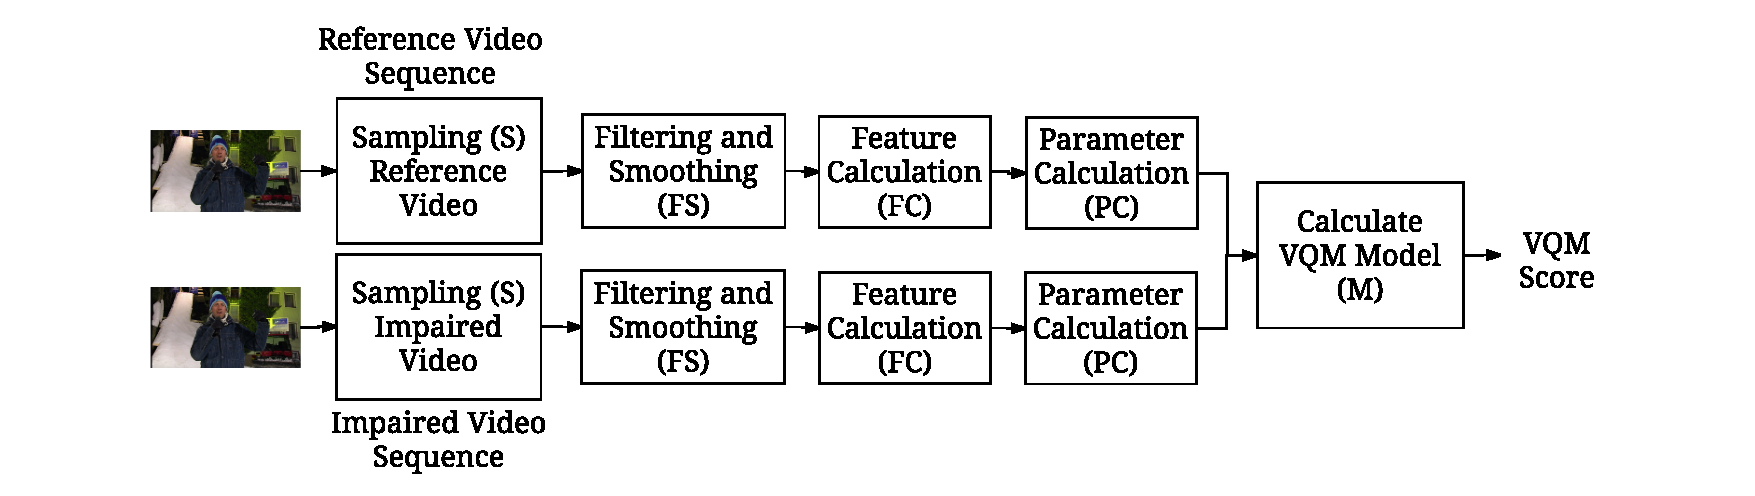
\includegraphics[width=\textwidth]{./gfx/200_Background/VQM_Steps}
	\caption[VQM assessment steps]{Essential steps of a VQM assessment inspired by Pinson et al.~\cite{Pinson2004}.}
	\label{fig:220_vqmsteps}
\end{figure}
 
Reference and impaired video sequence must have the same frame rate and resolution before they are decoded into the YCbCr color space.
This color space contains one luminance channel (Y) and two chrominance channels (CbCr).
The first step is \acf{S}, and it is conducted for each of the video sequences independently. 
\ac{S} converts each of the video frames into floating-point representations as it offers the required accuracy for a precise estimation of the perceived quality.

\acf{FS} applies the Sobel edge filter to the synchronized frames of the reference and the impaired video~\cite{Sobel1968}. 
To analyze the quality degrading changes, an edge difference metric is calculated for a spatial metric, and a temporal metric is computed for detecting degradations.

The \acf{FC} step determines visual features in a single video frame and across frames, which are combined in an \acf{ST-Region}.
It pans across $8\times8$ pixels and $6$ frames at a frame rate of 30, i.e., 0.2 seconds of video.

Five different feature sets are extracted from the \ac{ST-Region}, including two features that focus on structural information 
whereas the others address color information,
contrast, 
and motion. 
The resulting \ac{ST-Region}s from both representations are compared by the \ac{PC} step, resulting in an \ac{ST-Region} error matrix quantifying the differences between both videos.
Afterwards, the errors of each feature across the \ac{ST-Region}s are condensed into a single value - and for different \ac{ST-Region}s. 
A linear regression model determines the resulting \ac{VQM} value in a \acf{M} step.
The regression models were validated in extensive subjective studies. 
The \ac{VQM} values range from $0$ (reference video sequence) to 1 (impaired video sequence).

\ac{VQM} achieves high correlations with subjective experiments but requires a reference video for conducting the assessment.
At the same time, the runtime for processing is rather high, making it unusable for real-time applications.
\paragraph{VMAF}
\ac{VMAF} is the recently proposed recommendation of the video provider Netflix~\cite{Li2016}.

\ac{VMAF} leverages the strengths of different metrics to predict the perceived quality by fusing them using an \ac{SVM} regressor.
The \ac{SVM} regressor generates the weights on the impact of each metric on the final quality score.
The leveraged metrics comprise the Visual Information Fidelity metric, which measures the loss of information.
The second metric determines the loss of details and the loss of content visibility, which distracts viewers.
Both metrics measure the spatial impact of degradations.
Also, the impact of degradations on the motion is assessed by calculating the average absolute differences of the pixels on the luminance plane.

The learned model has shown to reliably detect compression and transmission artifacts for a broad range of datasets.
\paragraph{V-BLIINDS}
\ac{V-BLIINDS} is a \ac{NR} objective quality assessment algorithm combining spatial and temporal artifact detection and achieving comparable correlation rates with subjective studies~\cite{Saad2014}. 
The algorithm leverages the concept of natural scene statistics, which relies on the observation that undistorted videos show statistical regularities.
Irregularities in distorted videos allow a determination of the quality loss.
\ac{V-BLIINDS} leverages irregularities when representing motion in a video by using a \ac{DCT} representation of a video, or specifically of two consecutive frames. 
A joint spatial and temporal distortion detection and assessment is performed on the \ac{DCT} representation.
A two-dimensional spatial \ac{DCT} is applied on $n \times n$ pixel subblocks of a video frame.
Between two related subblocks, frequency differences are calculated.
From these differences, a statistical analysis is performed to detect irregularities from undistorted frequency coefficients.
\paragraph{Discussion}
Table~\ref{tab:video_quality_metrics_comparison} shows the performance of the algorithms regarding processing time for a $15$ second video and the correlation with subjective assessments. 
This correlation gives the capability of an objective quality metric to predict the perceived quality by an average human.
\begin{table}
	\centering 
	\caption[Comparison of objective video quality assessment algorithms]{Comparison of objective video quality assessment algorithms. The columns depict the metric classification, the algorithm execution time in seconds for analyzing $15$ seconds of video at a resolution of 720p and $30$ \ac{FPS} (lower is better), the \ac{SROCC} with subjective studies (CC, higher is better), and the metric's recommendation status.}
	\begin{tabular}{lcccccc}
		\textbf{Algorithm} &  \textbf{Type} & \specialcell{\textbf{Runtime} $[s]$ } &  \specialcell{\textbf{Correlation} \\ \textbf{LIVE DS}~\cite{Vu2011}}  & \specialcell{\textbf{Recommendation}}\\
		\midrule%\specialrule{1.5pt}{1pt}{1pt}
		PSNR      & FR      & 1.6    & 0.4035      & - \\
		SSIM~\cite{Wang2003}  & FR	& 104    & 0.658   & - \\
		VQM~\cite{Pinson2004} & FR / RR       & 88    & 0.770   & ANSI/ITU~\cite{ANSI2003,ITU2004} \\
		VMAF~\cite{Li2016} & FR & 198 & 0.872  & Netflix Inc. \\
		%BRISQUE~\cite{Mittal2012} & NR & ??? & ???  & ???? \\
		%MOVIE~\cite{Seshadrinathan2010}   & 2732  & 0.8116   & -\\
		V-BLIINDS~\cite{Saad2014} & NR & 14.2 & 0.759  & - \\
		%
		%(ST-)MAD~\cite{Chandler2010}   & 54876 & 0.8299  & no \\
		\midrule
	\end{tabular}
	\label{tab:video_quality_metrics_comparison}
\end{table}
The performance is measured on a commodity server\footnote{Hardware setup: Intel Xeon CPU E5-1650 with 64 GB of dedicated memory}.
The basis for our results is the LIVE video dataset, which contains ten \ac{720p} videos, each available in 15 distorted versions~\cite{Vu2011}. 
Each video has been manually annotated by a quality value by 38 subjects in controlled experiments.

An advantage of the simple \ac{PSNR} is the low execution time of $1.6$ seconds.
Due to the low correlation, the \ac{PSNR} is only the baseline for other algorithms.
None of the other \ac{FR} algorithms can perform a reliable estimation of the perceived quality in real-time, which is essential in live streaming.
An appropriate processing time for a live scenario is less than $15$ seconds. 
Especially, highly precise algorithms such as \ac{VMAF} and \ac{VQM} have execution times far beyond real-time capabilities.
\ac{VQM} was validated in large-scale user studies and standardized by the \ac{ANSI}/\ac{ITU}.
A recent modification of the \ac{VQM} algorithm allows to run it on a \ac{GPU}, which achieves the same correlation in real-time. This version, called \ac{RT-VQM}, has been co-developed by the author of this work, but is not discussed in this thesis~\cite{Wichtlhuber2016}. 

The \ac{VMAF}, as proposed by Netflix, relies on an \ac{SVM} for quality estimation. 
Once trained, the classification should be quickly achieved.
Still, the processing times are even higher than the ones for \ac{VQM}.
The discussed \ac{V-BLIINDS} algorithm achieves a considerable correlation at a low runtime.
The algorithm is thus suited for efficient \ac{UGV} assessment when no reference is present.
\subsection{Summary}
Findings can be gained from the previous discussion of the recording quality and the video quality.
Existing recording quality assessment algorithms detect degradations, but do not assess their impact on human perception.
Quality models are needed to fill the gap to not only detect a degradation, but also to allow one to assess its impact on the perceived quality.
Algorithms need to be redesigned to not only detect a degradation but also quantify the individual characteristics of each degradation.

In the live \ac{UGV} streaming scenario pursued in this thesis, a real-time assessment of the perceived quality is required.
The presented recording quality assessment and video quality assessment metrics are too slow for real-time processing.
Exceptions are algorithms that leverage auxiliary sensors to detect recording degradations.
They usually suffer from a reduced correlation with subjective studies and have to cope with noise in the sensor readings.
Approaches need to be found to improve the speed of the algorithms while keeping a high correlation with subjective studies. 

Existing algorithms discuss the assessment of a single video stream.
None of the algorithms addresses how to scale the quality assessment to multiple video streams, as, e.g., needed in the video composition proposed in the thesis.
